\chapter{Expected Nodes: communautés de liens dans les graphes statiques}
\minitoc

Les structures communautaires dans les graphes ont été beaucoup étudiées lorsque la structure concerne les n\oe uds mais également, dans une moindre mesure, pour les liens.
Les partitions de n\oe uds d'un graphe trouvent leurs limites lorsque les communautés se chevauchent.
Dans ce cas, il est plus intéressant à ce que chaque n\oe uds puisse appartenir à plusieurs communautés.
On manipule alors une partition chevauchante ou couverture.
Pour répondre à ce problème de nombreux algorithmes ont été proposés pour la détection et l'évaluation de couvertures de n\oe uds.
Cependant les couvertures, en tant que généralisation des partitions, sont encore plus difficiles à évaluer que les partitions.
Les partitions de liens, quant à elles, restent des objets plus simple à manipuler.
De plus, elles permettent de mettre en avant une autre structure ayant également du sens.

Dans un réseau sociale, chaque personne a plusieurs centres d'intérêts: famille, sport, politique...
Lorsque deux personnes sont communiquent, la communication a lieu dans un contexte bien particulier.
Bien que les personnes ont plusieurs centres d'intérêts, la raison de la communication est unique.
Il semble donc qu'une information importante soit intrinsèquement liée au lien.
Via la recherche de partitions de liens d'un graphe, c'est cette information que nous cherchons à capturer.

Il apparait donc les partitions de liens sont des objets à part entières pertinent à étudier.
Il est alors nécessaire d'adapter les outils d'analyses pour évaluer directement les partitions de liens.
Nous développons ici une approche similaire à ce qui est fait pour les partitions de n\oe uds et la modularité~\cite{Newman2004}.
Le but est de créer une fonction de qualité permettant d'évaluer une partition de liens d'un graphe.


\section{Travaux existants}
Les notations utilisées sont les suivantes. Soit $G=(V,E)$ un graphe non-orienté avec $V$ l'ensemble des n\oe uds de taille $n$ et $E \subseteq V \times V$ l'ensemble des liens de taille $m$. 
Le degré d'un sommet $u$ de $G$ est noté $d_G(u)$.
Une partition des liens en $k$ groupes est notée $\mathcal{L}=(L_1,L_2,\ldots,L_k)$ avec $L_i \subseteq E \ \forall i$, $L_i\cap L_j=\emptyset \ \forall i\neq j$ et $\bigcup_i L_i=E$.
Pour un groupe de liens $L \in \mathcal{L}$, on pose $V_{in}=\{u \in V, \exists (u,v) \in L\}$ l'ensemble des n\oe uds internes au groupe $L$, $V_{out}=\{u \in V\setminus V_{in}, (u,v) \in E \wedge v \in V_{in} \}$ représente les n\oe uds adjacents au groupe $L$ et enfin $L_{out}=\{(u,v) \in E \setminus L, u \in V_{in} \vee v \in V_{in} \}$ l'ensemble des liens adjacents au groupe $L$ (voir Figure~\ref{fig:example_def_expected}).

\begin{figure}
\centering
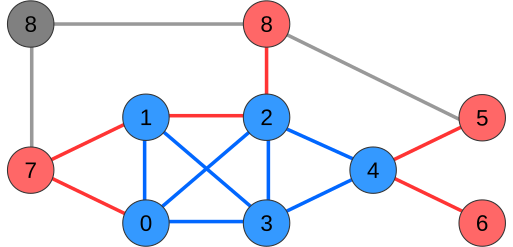
\includegraphics[width=0.4\linewidth]{img/ExpectedNodes/exemple2}
\caption{Exemple d'un groupe de liens $L$ (en \textcolor{semilightblue}{bleu}). Les liens \textcolor{pinkyred}{rouges} sont les liens adjacents $L_{out}$ connectant les n\oe uds internes $V_{in}$ (en \textcolor{semilightblue}{bleu}) aux n\oe uds adjacents $V_{out}$ (en  \textcolor{pinkyred}{rouge}).}
\label{fig:example_def_expected}
\end{figure}

Il existe différent type de méthodes existantes.
Il y les méthodes évaluant une partition de liens via la transformation de la partition en une couverture de n\oe uds~\cite{Huang2013,Lim2014,Wu2010a}.
Il serait tentant de considérer que les partitions de liens et les couvertures de liens sont équivalentes.
Ainsi pour évaluer une partition de liens, il suffirait de transformer la partition en couverture.
Or, ce changement n'est pas anodin.
D'une part, les couvertures de n\oe uds permettent de modéliser beaucoup plus de situations car il n'y a aucune contrainte sur les couvertures.
D'autre part, il n'est pas trivial de transformer une partition de liens en couverture de n\oe uds, et \emph{vice versa}.

\begin{figure}
\centering
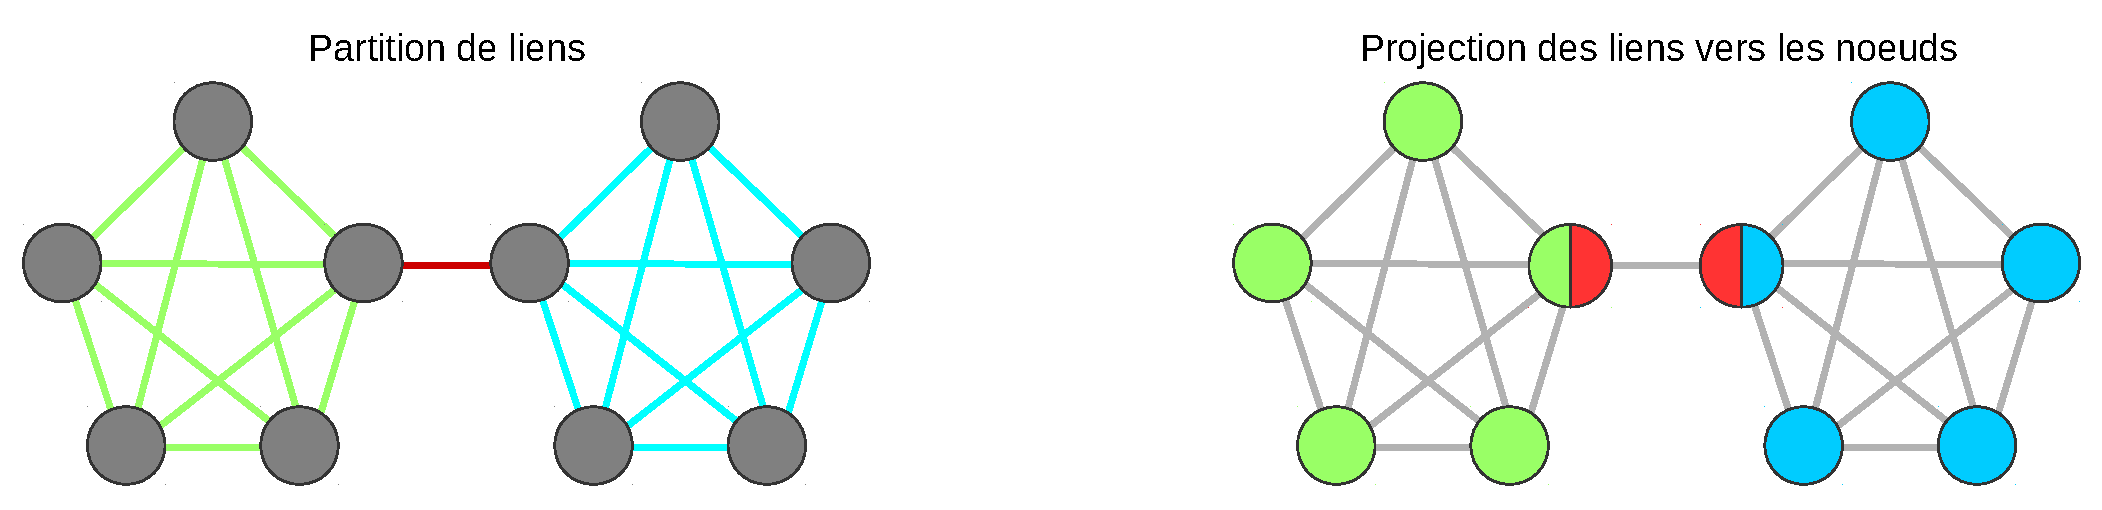
\includegraphics[width=0.9\linewidth]{img/ExpectedNodes/Partition_Couverture}
\caption{Transformation d'une partition de liens à gauche en couverture de n\oe uds à droite. La couleur représente un groupe.}
\label{fig:Partition_Couverture}
\end{figure}

Dans la figure~\ref{fig:Partition_Couverture}, est présenté une transformation basique d'une partition de liens en une couverture.
Dans cette transformation, un n\oe uds dans la couverture prends comme communauté l'ensemble des communautés de ses liens.
Dans cet exemple, il est évident que la communauté rouge consitutée des deux n\oe uds centraux n'est pas une communauté légitime et qu'il s'agit d'un artefact de la transformation.
La transformation d'une partition n'est donc pas un acte neutre.
Cet aspect a d'ailleurs était mis en avant par Esquivel~\emph{et al}~\ref{Esquivel2011}.
Face à ce problème, nos travaux ainsi que quelques méthodes existantes proposent des méthodes évaluant directement les partitions de liens.

Ahn \emph{et al.}~\cite{Ahn2010a} sont parmis les premiers à avoir proposé une méthode détectant les communautés de liens.
Leurs méthodes \emph{link clustering} est une méthode hiérarchique d'agglomération.
Elle construit un dendrogramme en agglomérant de manière itérative les groupes de liens en fonction de leurs similarités calculée par l'indice de Jaccard.
Afin de decider de la coupe du dendrogramme et de la partition résultantes, la fonction \emph{partition density} est utilisée.
Pour une partition de liens donnée $\mathcal{L}$, la \emph{partition density} est définie de la manière suivante:
\begin{equation}
D(\mathcal{L}) = \dfrac{\sum_{L \in \mathcal{L}} |L|D(L)}{m} \quad D(L) = \dfrac{|L|- min_D(|V_{in}|) }{max_D(|V_{in}|) - min_D(|V_{in}|)},
\end{equation}
Il s'agit de la moyenne pondéré de la qualité de chaque groupe.
La qualité d'un groupe est le nombre de liens du groupe normalisé par le nombre de liens minimum et maximum pour un groupe de $|V_{in}|$ n\oe uds.
Le nombre minimum de liens est obtenu par un arbre: $min_D(N) = N - 1$.
Le nombre maximum est obtenu par une clique: $max_D(N) = \dfrac{N(N - 1)}{2}$.\\
Aprés simplification, on obtiens la formule suivante:

\begin{equation}
 D(L) = 2 \dfrac{|L| - (|V_{in}|-1) }{(|V_{in}|-1) (|V_{in}|-2)}.
\end{equation}

D'autres chercheurs~\cite{Li2013,Shi2013} ont par la suite utilisé la \emph{partition density} comme fonction à optimiser dans un algorithme génétique.
Leurs solutions semblent pour l'instant difficile car leurs algorithme reposent sur de nombreux critères et limité à de petit graphes.

Par ailleurs, la \emph{partition density} ne peut pas être directement appliquée aux graphes pondérés.
Une première proposition a été faite par Kim~\cite{Kim2014}.


Evans~\emph{et al.}~\cite{Evans2009} propose trois fonctions de qualité pour évaluer les partitions de liens.
Leurs fonctions de qualité sont basées sur trois marches aléatoires qui se déroulent sur les liens du graphe.
L'approche est similaire à la modularité car la modularité peut également être définie à l'aide de marche aléatoire sur les n\oe uds du graphe~\cite{Delvenne2010}.
Leurs trois fonctions de qualités peuvent être calculées et optimisées sur le graphe mais les auteurs ont montré que l'on pouvait, de manière completement équivalente, utiliser la modularité sur des line graphe pondérés ($LG_1$, $LG_2$, $LG_3$).
Ainsi, il suffit de construire le line graphe approprié puis d'utiliser un algorithme existant d'optimisation de la modularité tel que l'algorithme de \emph{Louvain}~\cite{Blondel2008a}.
Un line graphe est un graphe où chaque lien du graphe initial est transformé en un n\oe uds dans le line graphe.
Deux n\oe uds du line graphe sont reliés si les liens correspondant ont au moins un n\oe uds en commun.

Pour construire les lines graphes  $LG_1$, $LG_2$ et $LG_3$, nous définissons $B\in \mathcal{M}_{n,m}$ la matrice d'incidence du graphe $G$: un élément $B_{i\alpha}$ de cette matrice $|V| \times |E|$ est égale à $1$ si le lien $\alpha$ est relié au n\oe uds $i$ et 0 sinon.
Les matrices $LG_1$, $LG_2$ et $LG_3$ sont alors définies de la manières suivantes:
\begin{center}
	\begin{tabular}{|c|c|c|c|}
		\hline  & $x=1$ & $x=2$ &  $x=3$\\ 
		\hline \rule{0pt}{1.8em} $LG_x(\alpha,\beta)$ & $B_{i\alpha}B_{i\beta} (1-\delta_{\alpha \beta})$ & $\sum_{i \in V, d_G(i)>1}\dfrac{B_{i\alpha}B_{i\beta}}{d(i)-1}$ & $\sum_{i,j \in V, d(i)d_G(j)>0}\dfrac{B_{i\alpha}A_{ij}B_{j\beta}}{d(i)d(j)}$ \\
		\hline 
	\end{tabular} 
\end{center}
Soit $k_x(\alpha)= \sum_{\beta}LG_x(\alpha,\beta)$ le degré pondéré dans le line graphe $LG_x$ du n\oe uds représantant le lien $\alpha$ et $W_x = \sum_{\alpha,\beta \in |E|}LG_x(\alpha,\beta)$ la somme des poids des liens. Pour $x \in \{1,2,3\}$, la fonction de qualité $Evans_x$ est définie de la manières suivante:
\begin{eqnarray}
Evans_x(\mathcal{L}) = \dfrac{1}{W_x} \sum_{L_i \in \mathcal{L}} \sum_{e_1,e_2 \in L_i^2} LG_x    (e_1,e_2) -  \dfrac{k_x(e_1) k_x(e_2)}{W}.
\end{eqnarray}

Kim \emph{et al.}~\cite{Kim2011} ont exploré une extension du concept \emph{Minimum Length Description} (MDL) introduit par Rosvall~\emph{et al.}~\cite{Rosvall2008} qui méthode provenant de la théorie de l'information.
Cette extension de la \emph{MDL} évalue directement une partition de liens, contrairement à l'extension proposée par Esquivel~\emph{et al.}~\cite{Esquivel2011}.
Un avantage de leur méthode est de pouvoir comparer l'avantage d'utiliser une partition de liens ou une partition de n\oe uds avec leur \emph{MDL} respective.
Cependant, leur méthode semble favoriser les communautés de liens que dans des cas très précis.


\section{Définition d'Expected Nodes}

Une idée souvent utilisée lors de la détection de communautés de n\oe uds est qu'une communauté devrait avoir beaucoup de connexion en interne.
Pour appliquer ce genre de définition intuitive, il est nécessaire de définir à quoi comparer le nombre de connexion interne.
Le choix qui est fait avec la modularité et d'autres méthodes est de définir un modèle nul aléatoire où il n'existe pas de structure communautaire.
Le but est de construire un graphe aléatoire qui partage un certains nombre de caractéristiques avec le graphe initial mais dont la structure a été détruite lors du mélange.

Il existe de nombreux modèles et celui utilisé dans la modularité est le modèle de configuration~\cite{Bender1978a}.
Dans ce modèle, le nombreux de n\oe uds et leur degré sont fixes mais la répartition des liens est aléatoire.
Ainsi pour chaque n\oe uds, ses voisins sont tirés de manière aléatoire avec une probabilité proportionnelle à leur degré.
Comme les liens sont mélangés dans ce modèle, on suppose qu'il n'existe plus de structure communautaire dans le graphe.

Pour notre fonction de qualité \emph{Expected Nodes}, nous utilisons également le modèle de configuration.
Avant d'aller plus loin et de définir formellement \emph{Expected Nodes}, il est utile d'avoir une définition informelle de la fonction de qualité.

Le but est d'évaluer un groupe de liens.
Afin qu'un groupe de liens soit évalué comme une bonne communauté, les liens devraient induire un nombre relativement faible de n\oe uds internes.
En effet, plus le nombre de n\oe uds internes est faible, plus le groupe de liens ressemble à une clique.
De manière similaire à la modularité, nous utilisons le configuration modèle pour calculer le nombre de n\oe uds interne espéré dans un modèle nul.
Si le groupe de liens a moins de n\oe uds internes qu'espéré alors ça indique que le groupe de liens est plus dense et qu'il devrait donc avoir une évaluation élevée.

Il est donc nécessaire de calculer l'espérance du nombre de n\oe uds interne, $\mu_{G}$, d'un groupe de liens, $L$, dans le modèle nul.
Un n\oe uds de $G$ est interne si au moins un de ses  demi-liens appartient à $L$.
Ainsi pour calculer $\mu_{G}$, il faut tirer aléatoirement et sans remise $2|L|$ demi-liens parmi les $2|E|$ demi-liens du  graphe aléatoire avec la m\^eme distribution de degrés.
Soit $B_u$ la variable aléatoire correspondant au nombre de fois où le sommet $u$ est tiré.
Cette variable suit une loi  hypergéométrique $B_u \sim \mathcal{G}\left(2|E|,d_G(u),2m\right)$.
Avec cette notation, on définie $\mu_G$ de la manière suivante:

\begin{equation}
\label{eq:nbsommet_esp} \mu_{G}(|L|) = \sum_{u\in V} \mathbb{P}( B_u \geq 1 )
=  \sum_{u \in V} 1 - \dfrac{ \binom{2|E|-d(u)}{2|L|} }{ \binom{2|E|}{2|L|} }. 
\end{equation}

Voici quelques propriétés de la fonction $\mu_{G}(|L|)$ :
\begin{itemize}
\item La fonction $\mu_{G}$ dépend uniquement de la séquence de degrés $\{d_G(v)\}_{v \in V}$. %\noe{ et du nombre d'arêtes}.
On peut montrer que cette fonction est Schur-concave, ainsi plus les degrés sont uniformément répartis plus il sera surprenant d'observer un groupe de liens correspondant à peu de n\oe uds.
\item Pour une distribution de degrés donnée, la fonction   $\mu_{G}(|L|)$ est une fonction croissante de $|E|$.
\item Si $L=E$, alors le nombre de n\oe uds attendus est bien $|V|$.
\item On a $\mu_{G}(1)\leq 2$, en effet le modèle nul n'interdit pas la présence de boucles.
\end{itemize}

Avec $\mu_G$, nous pouvons définir la qualité \emph{interne}, $Q_{in}$ d'un groupe de liens $L$:
  
\begin{equation}
\label{eq:qin} Q_{in}(L) = \dfrac{\mu_{G}(|L|) - |V_{in}(L)|}{\mu_{G}(|L|)}.
\end{equation}

Avec cette formulation, pour un groupe de taille $|L|$, plus le nombre de n\oe uds interne est faible, plus $Q_{in}$ sera élevée.

$Q_{in}$ permet d'évaluer la qualité interne d'un groupe mais il faut aussi tenir compte du voisinage.
C'est pourquoi, nous définissons également une qualité externe.
Le but est d'évaluer comment sont répartis les liens et n\oe uds adjacents.
Pour ce faire, nous allons également comparer le nombre de n\oe uds adjactens observés aux nombre espéré dans le configuration modèle.
Cependant à l'inverse de la qualité interne, la qualité externe est mauvaise si jamais le nombre de n\oe uds adjacent est plus faible qu'espéré.
En effet, si il y a beaucoup de liens adjacents pour peu de n\oe uds adjacents, alors cela indique que le voisinage du groupe est dense et devrait être inclus dans le groupe.
Le cas idéal est quand chaque lien adjacent est relié à un n\oe uds différent.

Soit $\bar{d}(L,u) = \sum_{v \in V} \mathbf{1}_{(u,v) \in E \setminus L}$ le degré de $u$ limité aux liens adjacents et $\bar{d}(L)=\sum_{u \in V_{in}(L)} \bar{d}(L,u)$.
L'espérance du nombre de n\oe uds adjacents est calculé comme le nombre de n\oe uds qui sont tirés lorsque $\bar{d}(L)$ demi-liens sont choisis aléatoirement et sans remise dans modèle de configuration où les liens de $L$ ont été préalablement retirés.
Ce graphe aléatoire a la distribution de degré suivante: $\{d_{G \setminus L }(u)\}_{u \in V}$ où $G \setminus L = (V,E\setminus L)$.
Dans ce cas, on ne tire pas aléatoirement un lien mais uniquement un demis-liens car l'autre demi-lien est un des demi-liens reliés aux n\oe uds internes.
L'espérance du nombre de n\oe uds adjacents se définit de la manière suivante:

\begin{equation}
	\mathbb{E}[\bar{d}(L)] = \mu_{G\setminus L}(\bar{d(L)}/2).
\end{equation}

Une illustration de ce processus est présentée dans la figure~\ref{fig:retourt_ext}.
Sur cette illustration, le groupe $L$ a un très mauvais voisinages et cela se reflète par un nombre de n\oe uds adjacents observés plus faible qu'espéré.

\begin{figure}
\centering
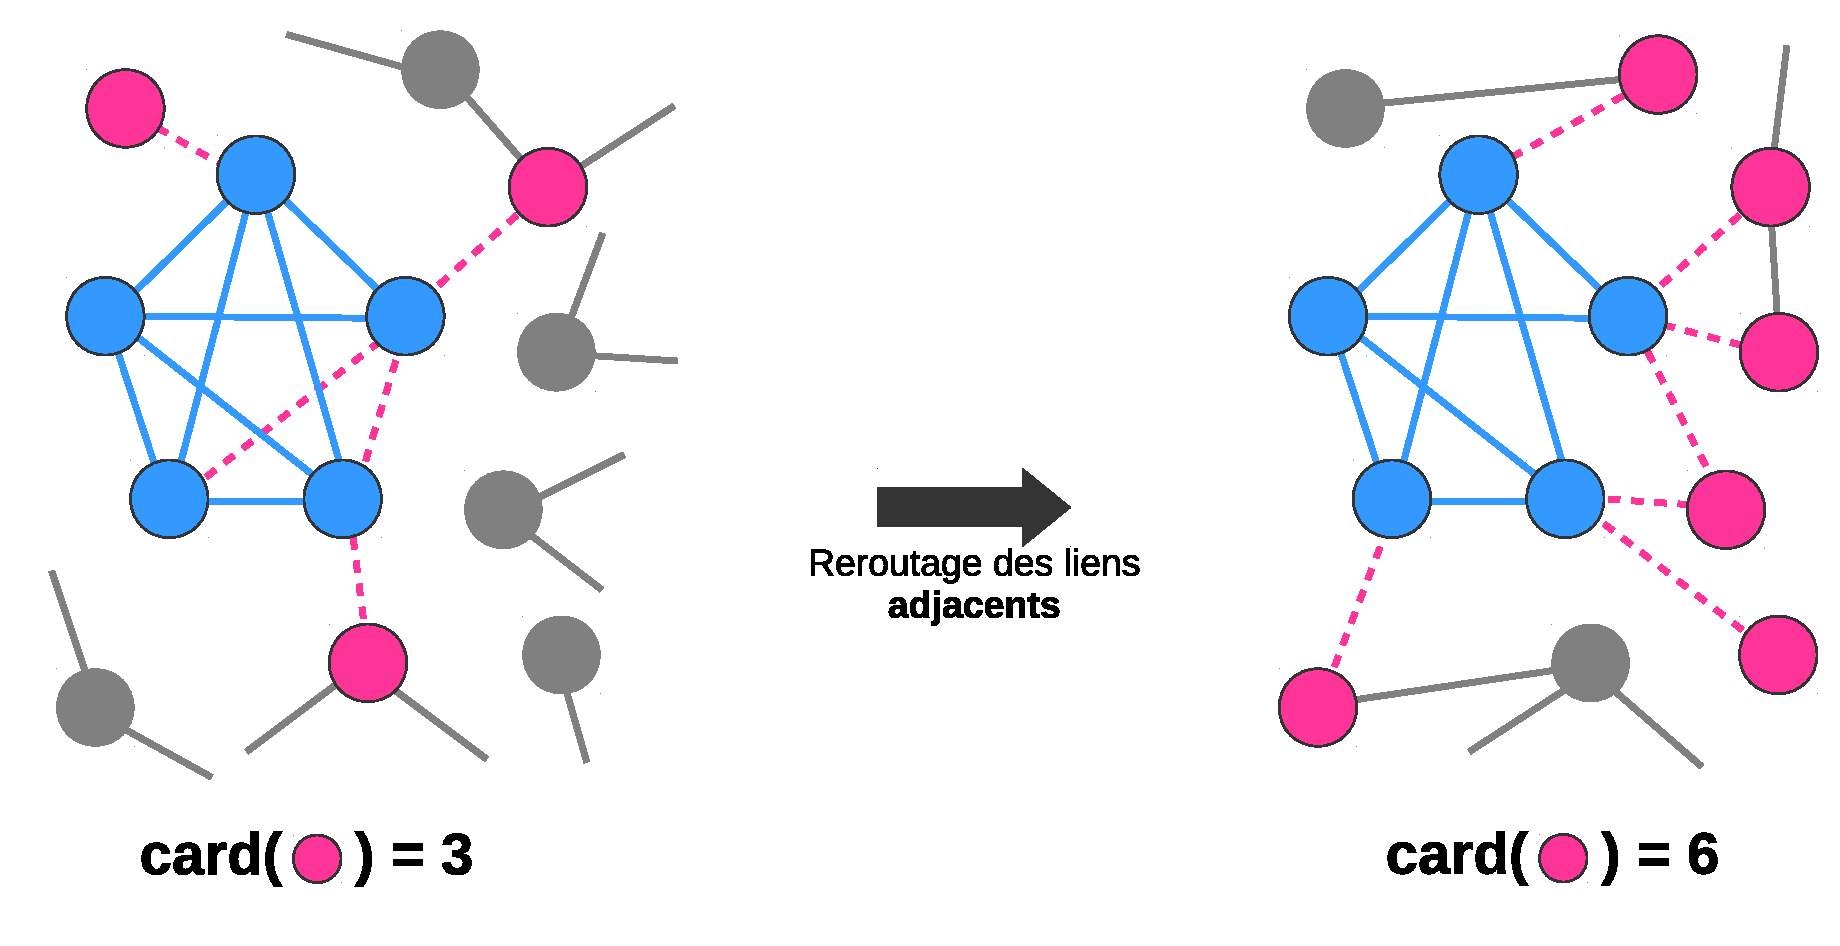
\includegraphics[width=0.7\linewidth]{img/ExpectedNodes/reroutageExt3}
\caption{Groupe de liens $L$ en \textcolor{semilightblue}{bleu} et ces liens adjacents en \textcolor{pinkyred}{rouges} dans le graphe initial à gauche.
\`A droite, une réalisation du modèle de configuration où $L$ a été figé.}
\label{fig:retourt_ext}
\end{figure}

Comme il est intéressant de pénaliser les groupes ayant de mauvais voisinage mais qu'un bon voisinage n'est pas suffisant pour définir une bonne communauté, nous bornons à $0$ la qualité externe:

\begin{equation}
\label{eq:qext} Q_{ext}(L) = min \left(0, \dfrac{|V_{out}(L)| - \mu_{G\setminus L}(\bar{d}(L)/2)}{\mu_{G\setminus L}(\bar{d}(L)/2)} \right).
\end{equation}


Enfin, nous définissons \emph{Expected Nodes} pour un groupe $L$:
\begin{equation}
	\label{eq:qAlg}
	Q(L)  =  2\dfrac{ |L|Q_{in}(L) + |L_{out}|Q_{ext}(L)}{|L|+|L_{out}|}.
\end{equation}

Nous utilisons la moyenne pondérée entre la qualité interne et externe car la qualité interne est dû aux liens de $L$ et la qualité externe par les liens adjacents.
Nous détaillons certaines propriétés des formules \ref{eq:qext} et \ref{eq:qAlg} découlant des propriétés de $\mu_{G}$ :
\begin{itemize}
\item En s'intéressant aux n\oe uds adjacents $V_{out}$, on pénalise la présence de n\oe uds adjacents fortement connectés avec les n\oe uds incidents à $L$.
\item Ainsi la qualité d'un lien isolé dépend du nombre de triangles dans laquelle il se trouve. Un lien séparant deux groupes de n\oe uds disjoints peut avoir une qualité positive.
\item La qualité du groupe contenant tout les liens est nulle.
\end{itemize}

Nous définissons \emph{Expected Nodes} pour une partition de liens $\mathcal{L}$ comme la moyenne pondérée de la qualité de chaque groupe:
\begin{equation}
\label{eq:qualite_globale} Q_G(\mathcal{L}) = \dfrac{\sum_{L\in \mathcal{L}} |L|Q(L)}{|E|}.
\end{equation}



\section{Comparaison}

Nous évaluons maintenant \emph{Expected Nodes} en utilisant deux jeux de test.
Sur ces jeux de tests, nous appliquons également des fonctions de qualités reconnues:
\emph{partition density}~\cite{Ahn2010a} et les fonctions de qualité proposées par Evans \emph{et al.}~\cite{Evans2009} que nous nommons $Evans1$, $Evans2$ et $Evans3$.
Pour chaque graphe de test, nous créons empiriquement plusieurs partitions de liens et nous évaluons chaque partition avec toutes les fonctions de qualité.

\subsection{Cas du graphe complet}
\label{Completegraph}
Le premier jeu de test est assez simmple puisqu'il s'agit d'un graphe complet.
Le but est de vérifier que \emph{Expected Nodes} n'ai pas un comportement dégénéré.
Nous étudions un graphe complet de $100$ n\oe uds\,\footnote{Nous avons obtenus des résultats similaires pour un graphe de $500$ n\oe uds.}.
Sur ce graphe, nous définissons plusieurs partitions.
La première est une partition triviale où tout les liens sont dans un unique groupe.
Nous définissons deux familles de partitions: une séparant les liens en deux groupes et une séparant les liens en 3 groupes.
Soit $V'$ un ensemble de $p$ n\oe uds où $p$ est un paramètre $p<|V|$.
Les deux familles de partitions placent les liens de $V' \times V'$ dans un groupe.
Pour la partition en 2 groupes, tout les autres liens sont mis dans un second groupe.
Pour la partition en 3 groupes, les liens de $V \times V\setminus V'$ sont dans un second groupe et le reste dans un troisième.
Ces répartitions sont illustrées dans la figure~\ref{fig:1C}.
%The group of a link $(u,v)$ is determined by the membership of $u$ and $v$ to $V'$ as illustrated in Figure~\ref{fig:1C}.
%\begin{table}
%	\begin{center}
%	\begin{tabular}{|c|c|c|c|c|}
%		\hline \backslashbox{Partition}{Link} & $u \in V' \wedge v \in V'$ & $u \in V' \wedge v \in V\setminus V'$ & $u \in V\setminus V' \wedge v \in V\setminus  V'$  \\ 
%		\hline 2 groups &  $a$ &  $b$ &  $b$ \\ 
%		\hline 3 groups &  $a$ &  $b$ &  $c$ \\ 
%		\hline		
%	\end{tabular}
%	\caption{Group assignment rule for a link according to the nodes attached to the link and given $V'$, a subset of $V$.}
%	\label{tab:ex1}
%	\end{center}
%\end{table}
%
%

\begin{figure}
\centering
	\subfloat[\label{fig:1C2}]{
		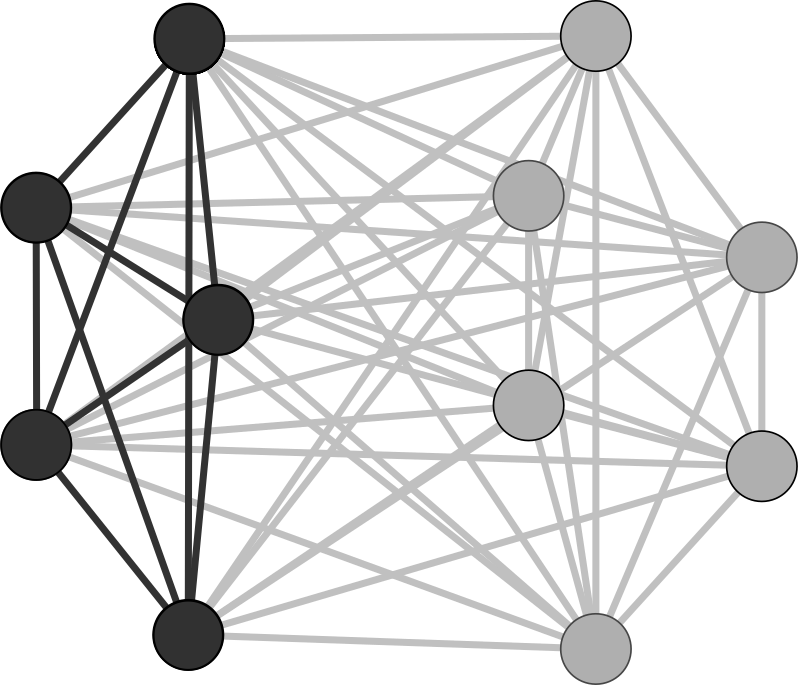
\includegraphics[width=0.2\linewidth]{img/ExpectedNodes/1Clique/Clique2}
	}
	\hspace{2cm}
	\subfloat[\label{fig:1C3}]{
		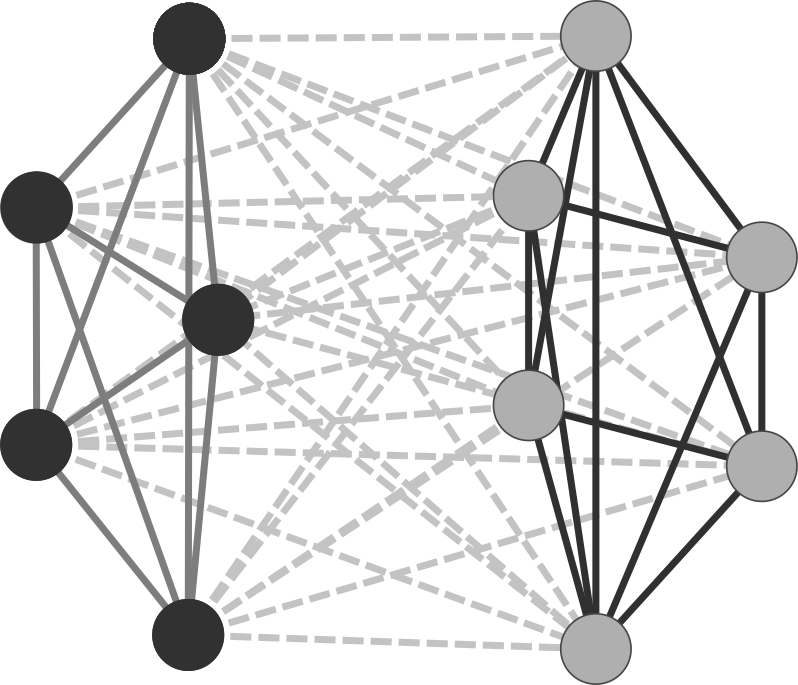
\includegraphics[width=0.2\linewidth]{img/ExpectedNodes/1Clique/Clique3}
	}
	\caption{Deux partitions de liens pour un graphe complet à $10$ n\oe uds avec $p=5$: (a) partition en deux groupes et (b) partition en trois groupes.
	Les n\oe uds noirs sont les n\oe uds appartenant à $V'$ et la couleur d'un lien correspond à son groupe.}
	\label{fig:1C}
\end{figure}

Comme le graphe est un graphe complet, la meilleur solution est d'avoir un seul groupe contenant l'ensemble des liens, \textit{i.e.} la partition triviale devrait avoir une meilleur évaluation que les autres partitions.
La figure~\ref{fig:1Cres} présentent les résultats.
Pour chaque valeur de $p$ et chaque fonction de qualité, nous calculons les évaluations des partitions en deux et en trois groupes ainsi que l'évaluation de la partition triviale.
L'évaluation de la partition trivial n'est pas dépendante de $p$ et est calculée qu'une seule fois.
De manière assez surprenante, les fonctions $Evans1$ et $Evans2$ ne passent pas ce test car elles évaluent la partition en deux ou trois groupes comme meilleur que la partition trivial.
Selon la \emph{partition density}, \emph{Expected Nodes} et $E_3$, la partition trivial est la meilleur des partitions.
La fonction $Evans3$ diffère légerement car elle a une amplitude plus faible ($\approx 10^{-3}$).
%On this example, the method link clustering and the method which optimizes $E3$ capture the ground truth where all the links are in a single community.
\begin{figure}
\centering
		\subfloat[\label{fig:1CAhn}\emph{Partition density}]{
			\includegraphics[width=0.49\linewidth]{img/ExpectedNodes/1Clique/Clique_Partitiondensity.eps}
		}
		\subfloat[\label{fig:1CE2}\emph{Evans1, Evans2}]{
			\includegraphics[width=0.49\linewidth]{img/ExpectedNodes/1Clique/Clique_Evans1.eps}
		}
		
		\subfloat[\label{fig:1CE3}$Evans3$]{
			\includegraphics[width=0.49\linewidth]{img/ExpectedNodes/1Clique/Clique_Evans3.eps}
		}		
		\subfloat[\label{fig:1CMod} \emph{Expected Nodes}]{
			\includegraphics[width=0.49\linewidth]{img/ExpectedNodes/1Clique/Clique_Expectednode.eps}
		}
		
		\caption{\`Evaluation des 5 fonctions de qualité sur un graphe complet  de $100$ n\oe uds pour trois type de partitions.
		Les partitions testées sont présenté dans la section~\ref{Completegraph}.
		Par définition, les résultats pour $Evans1$ et $Evans2$ sont identiques.
		Les lignes en gris, noir et pointillé représente respectivement la partition triviale, les partition en deux groupes et les partitions en trois groupes.}
		\label{fig:1Cres}
\end{figure}


\subsection{Graphe LFR}

Nous utilisons maintenant un jeu de test plus évolué.
Il n'existe pas à notre connaissance de générateur de graphe aléatoire avec une structure communautaire sur les liens.
C'est pourquoi, nous utilisons le générateur proposé par Lancichinetti \textit{et al.}~\cite{Lancichinetti2009b}.
Ce générateur aléatoire permet de générer des graphes ayant une structure communautaire chevauchante sur les n\oe uds.
Comme nous voulons évaluer une partition de liens, il est nécessaire de transformer cette vérité de terrain.
Nous introduisons deux transformations de la couverture des n\oe uds en deux partitions de liens, $TA$ et $TB$, voir figure~\ref{fig:Trans}.

Soit $u,v \in V$, $C_{u,v}$ désigne l'intersection des communauté de $u$ et $v$ dans la couverture et $U_{u,v}$ désigne leur union.
Nous définissons le groupe d'un lien $(u,v) \in E$ dans $TA$ et $TB$ de la manière suivante:
\begin{description}
\item[\textbf{intra-communauté}] si $|C_{u,v}| = 1$ alors $(u,v)$ est dans la communauté $C_{u,v}$;
\item[\textbf{inter-communauté}] si $|C_{u,v}| = 0$ alors dans $TA$, $(u,v)$ appartient à sa propre communauté.
Dans $TB$, le liens appartient à la communauté $U_{u,v}$, qui contient l'ensemble des liens $(u',v')$ tel que $U_{u',v'}=U_{u,v}$;
\item[\textbf{chevauchement}] si $|C_{u,v}| > 1$ alors le lien $(u,v)$ appartient aléatoirement à une des communautés appartenant à $C_{u,v}$.
\end{description}

\begin{figure}
\centering
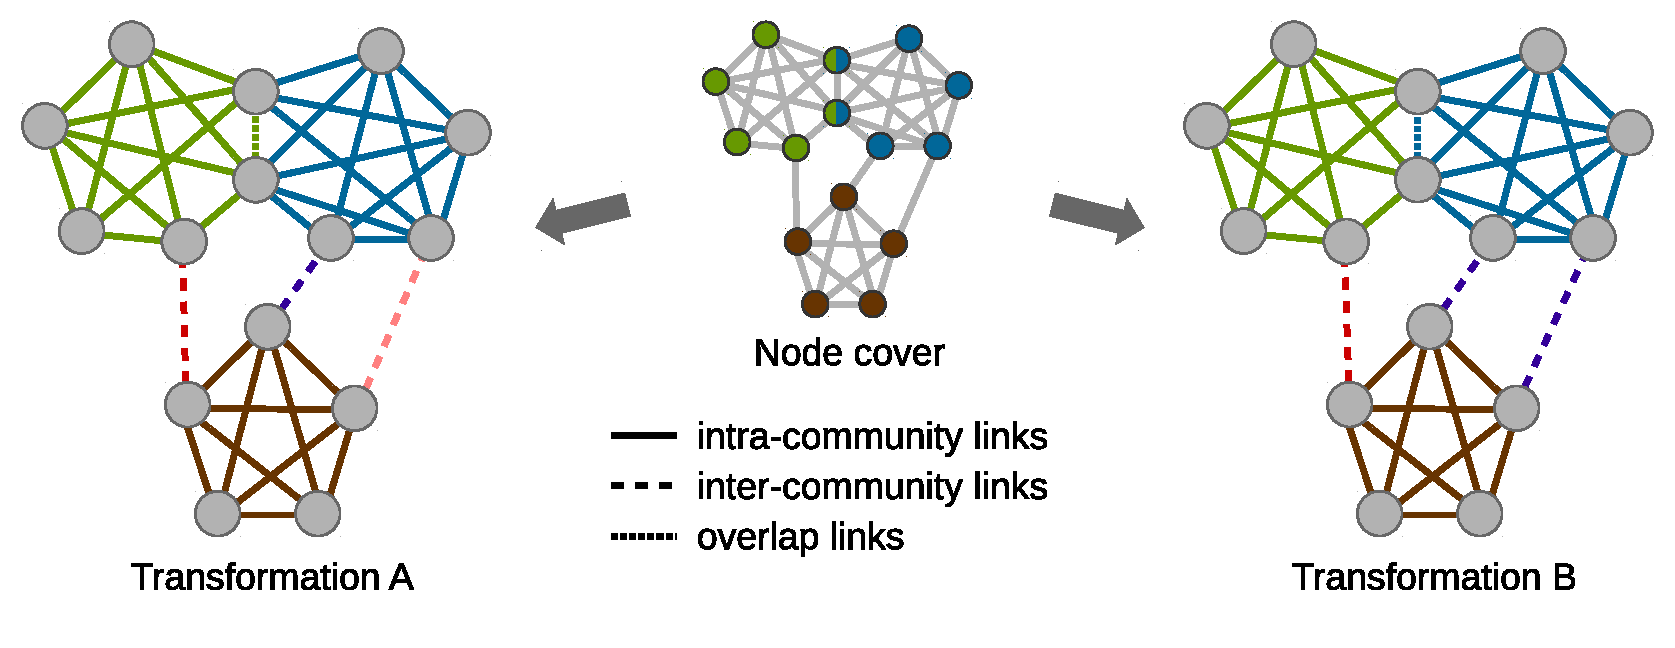
\includegraphics[width=0.9\linewidth]{img/ExpectedNodes/Example/GroundTruthTransformation}
\caption{Construction de $TA$ et $TB$ depuis une couverture de n\oe uds.
La couleur des liens indique leur groupe.}
\label{fig:Trans}
\end{figure}

Pour générer le graphe, nous avons appliqué un jeu de paramètre classiquement utilisé dans la littérature~\cite{Fortunato2010}.
Ainsi, nous avons généré des graphes de $500$ n\oe uds ayant un degré moyen de $25$, un degré max de $50$ et $10$ n\oe uds appartenant à deux communautés et des communautés ayant une taille comprise entre $20$ et $100$.
Le degré est tiré selon une loi exponentielle de paramètre $-2$ et la taille des communautés a $-1$ comme paramètre.
Enfin, 90\% des liens se sont à l'intérieur d'une communauté et les 10\% restant sont répartis de manière aléatoire.
Avec ces paramètres, il y a en moyenne $5620$ liens intra-communautés, $625$ liens inter-communauté et seulement $5$ liens chevauchant.

Pour chaque graphe généré, nous testons les partitions $TA$ et $TB$ mais aussi la partition $LC$ trouvée par \textit{link clustering}~\cite{Ahn2010a} et la partition $E2$ trouvée par la seconde méthode de Evans \textit{et al.}~\cite{Evans2009}\,\footnote{The results are similar for the algorithms using $E1$ and $E3$.}.
Ces deux algorithmes optimisent respectivement \emph{Parition Density} et \emph{Evans2}.
Ces partitions sont ensuite évaluées par les fonctions de qualité \emph{Partition Density}, $Evans2$ et \emph{Exoected Node}.
Une illustration d'un graphe généré et des exemples de groupes capturées par $LC$ et $E2$ sont présentés dans la figure~\ref{fig:LFR_Exemple}.

\begin{figure}
\centering
	\subfloat[]{
				\includegraphics[width=0.31\linewidth]{img/ExpectedNodes/LF/Graphe_Complet_select.png}
	}
	\subfloat[\label{fig:LFR_ExempleE2}]{
		\includegraphics[width=0.31\linewidth]{img/ExpectedNodes/LF/E2_bis.png}
	}			
	\subfloat[\label{fig:LFR_ExempleLC}]{
		\includegraphics[width=0.31\linewidth]{img/ExpectedNodes/LF/Ahn.png}
	}

	\caption{Exemple de graphe généré par le LFR en (A) avec une communauté de la vérité de terrain mise en avant en vert.
	En (B) zoom sur une communauté détectée par $E2$ dont les liens sont en verts.
	En (C) zoom sur une communauté détectée par $LC$ dont les liens sont en verts. }
	\label{fig:LFR_Exemple}
\end{figure}


Dans $LC$, $TA$, $TB$ et $E2$, il y a $720$, $650$, $70$ et $11$ groupes en moyenne.
Afin d'observer la ressemblance de ces partitions, nous avons utilisé la NMI~\cite{Danon2005}.
Il apparait que les partitions $TA$ et $TB$ sont les plus proches.
Ensuite, nous remarquons que la partition $E2$ diffère de $TA$ et de $TB$ uniquement sur les liens inter-communautés.
En effet si ils ne sont pas pris en compte lors de la comparaisons, alors $E2$, $TA$ et $TB$ sont équivalentes.
Il semble en effet que les liens inter-communautés soient arbitrairement distribués entre les plus grosses communauté adjacentes, ce qui est visible dans la figure~\ref{fig:LFR_ExempleE2}.
Enfin, la partition $LC$, bien que proche de $TA$ et $TB$, est un peu plus différente.
Ces $720$ groupes semblent plus petit mais aussi plus denses que ceux de $TA$ ou $TB$.
En particuluer, les liens intra-communautés peuvent être séparés dans plusieurs groupes, comme dans la figure~\ref{fig:LFR_ExempleLC}.
Les quatres partitions sont donc différentes et mettent en avant différentes caractéristiques.

Nous procédons maintenant à l'évaluation de ces partitions par les différentes fonctions de qualités.
Comme le processus de génération de graphe est aléatoire, les évaluations présentées dans la figure~\ref{fig:LF} représentent $30$ générations.
On remarque tout d'abord que ni $TA$ ni $TB$ n'a la meilleur évaluation selon $Evans2$ (figure ~\ref{fig:LFE2}) ou \emph{Partition density} (figure ~\ref{fig:LFAhn}) même si $TA$ et $TB$ représente nos vérités de terrains.
Dans le cas de \emph{Partition Density}, $TA$, $TB$ et $LC$ ont quasiment la même évaluation alors qu'il s'agit de structures assez différentes.
Dans le cas de $Evans2$, c'est la partition $E2$ qui obtient la meilleur évaluation.
Cela prouve l'efficacité de l'algorithme $E2$ pour optimiser $Evans2$ mais remets en cause la pertinence du critère $E2$ pour mettre en avant la vérité de terrain.
Enfin les partitions $TA$ et $TB$ ont encore une fois la même évaluation.
Notre fonction \emph{Expected Nodes} se comporte différemment des 2 autres.
Tout d'abord, c'est la vérité de terrain $TA$ qui obtient la meilleure évaluation puis il s'agit de $TB$ ou $LC$ selon les générations.
Notre mesure semble donc bien mettre en avant la vérité de terrain générée.
De plus, \emph{Expected Nodes} évalue différemment les partitions $TA$ et $TB$.
C'est un point important car, dans la partition $TB$, les liens inter-communautés peuvent donner lieu à des groupes non-connexes dans $TB$, voir figure~\ref{fig:Trans}.
Ce phénomène est très pénalisé par \emph{Expected Nodes}.
La partition $E2$ obtient une mauvaise évaluation également à cause des liens inter-communautés.
En effet en les fusionnant à une communauté adjacente, cela augmente fortement le nombre de n\oe uds interne ce qui fait baisser $Q_{in}$ mais $Q_{ext}$ baisse également.

Pour ces raisons, nous pensons que \emph{Expected Nodes} est une mesure qui permet de mieux évaluer les partitions de liens.

\begin{figure}
\centering
	\subfloat[\label{fig:LFAhn}Partition density]{
				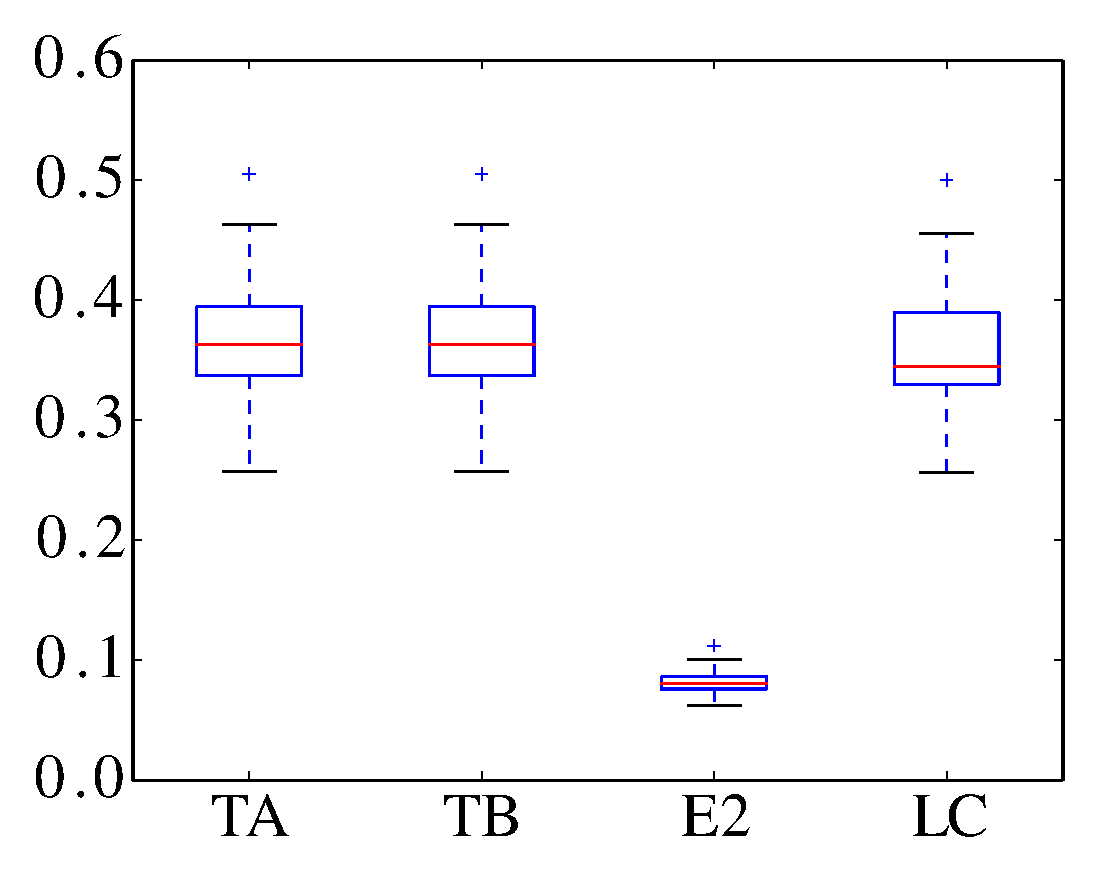
\includegraphics[width=0.31\linewidth]{img/ExpectedNodes/LF/LFR1_Partitiondensity_ALL.eps}
	}
	\subfloat[\label{fig:LFE2}Evans2]{
		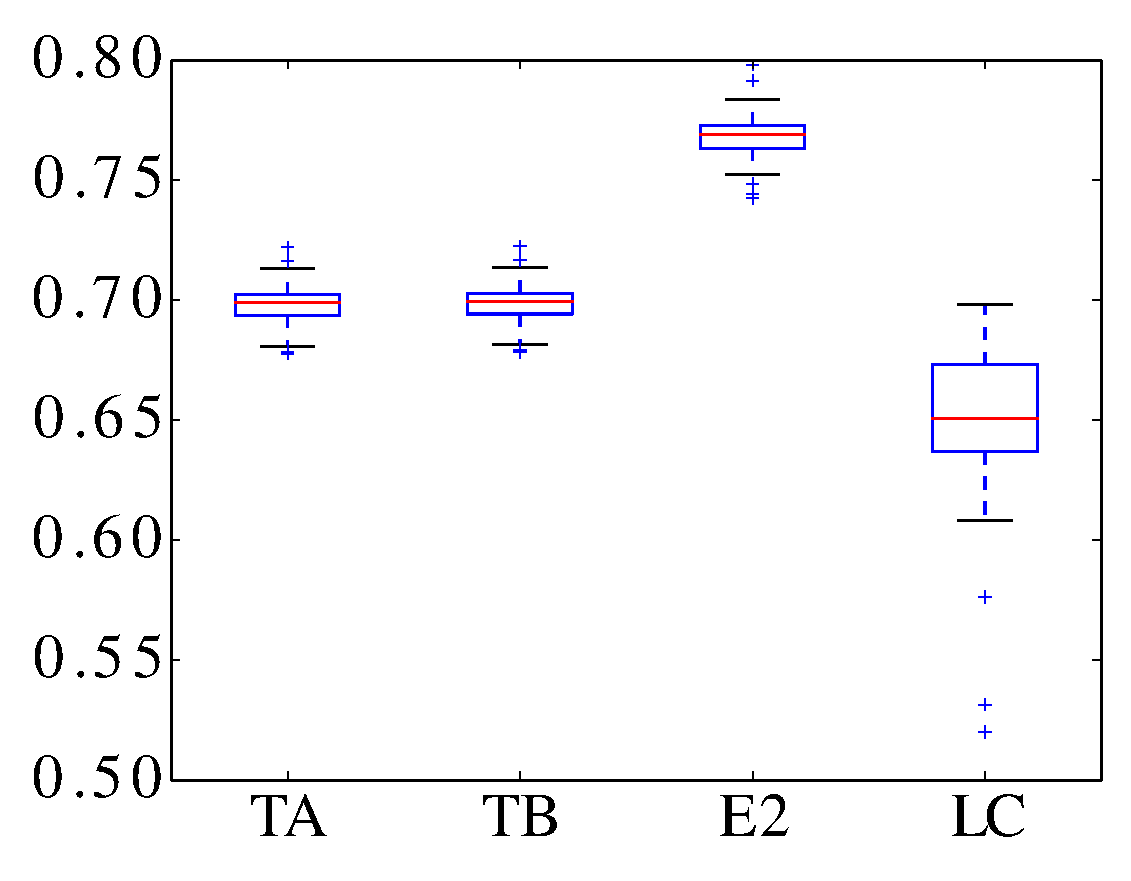
\includegraphics[width=0.31\linewidth]{img/ExpectedNodes/LF/LFR1_Evans2_ALL.eps}
	}			
	\subfloat[\label{fig:LFMod}Expected Nodes]{
		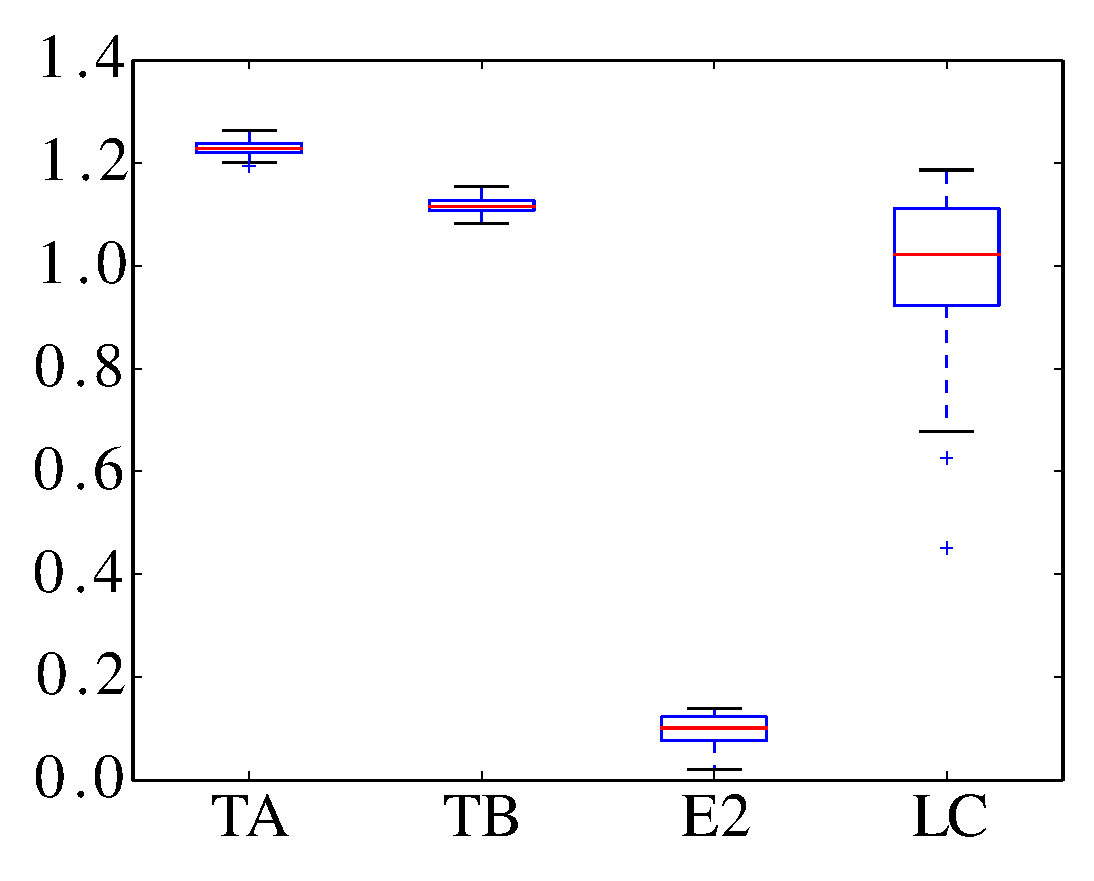
\includegraphics[width=0.31\linewidth]{img/ExpectedNodes/LF/LFR1_ExpectedNodes_ALL.eps}
	}

	\caption{Boite à moustache des évaluations des trois fonctions de qualité pour les différentes partitions de liens. 
	La boite représente le premier et troisième quartile ainsi que la médiane.
	Les moustaches s'étendent sur $1.5$ fois l'écart interquartile. 
	Les croix sont les points au delà des moustaches.
	}
	\label{fig:LF}
\end{figure}

\section{Calcul et optimisation}
Jusqu'à maintenant, nous avons évalué la mesure sans nous attacher ni à son calcul ni à son optimisation.
Nous discutons maintenant de la complexité de calcul d'\emph{Expected Nodes} pour une partition donnée.
Le calcul de la qualité interne \ref{eq:qin} nécessite d'évaluer la probabilité qu'un n\oe uds soit tiré.
Or, cette probabilité ne dépends que du degré du n\oe uds et du nombre de liens dans le groupe.
Donc, tout les n\oe uds ayant le même degré donnent lieu à la même probabilité.
Ce calcul de probabilité nécessite d'évaluer pour un n\oe uds $u$: $1 - \dfrac{ \binom{2|E|-d(u)}{2|L|} }{ \binom{2|E|}{2|L|} }$, ce qui peut être assez couteux.
Ce calcul correspond à une loi hypergéométrique.
Or sous certaines conditions, une loi hypergéométrique peut être approché par une loi binomial ce qui simplifie le calcul à: $1 - (1- \dfrac{|L|}{|E|})^{|L|}$ ce qui est plus rapide.
Lors de nos tests, le biais induit par cette approximation reste assez faible, de l'ordre de $0.01\%$ en moyenne.
Ce changement de calcul est équivalent à considérer un tirage avec remise au lieu de tirage sans remise.

Si l'on considère que l'évaluation de la probabilité peut se faire en $O(1)$ alors, pour un groupe donné, il est possible de calculer sa qualité en $O(|\{d_G(v)\}_{v \in V}|)$.
Cette propriété est très pratique lorsque beaucoup de n\oe uds ont le même degré.
Enfin comme la qualité d'un groupe ne dépend que de sa taille, on peut calculer la qualité d'une partition $\mathcal{L}$ en $O(\{|L_i|\}_{L_i \in \mathcal{L}})$.

Il est donc assez rapide de calculer $Q_{in}$.
En revanche, la situation est complètement différente pour $Q_{ext}$.
Le processus de calcul est similaire.
On peut de nouveau appliquer l'approximation de la loi hypergéométrique par une loi binomiale mais deux n\oe uds de même degré ne vont plus forcément avoir la même probabilité d'être tiré.
En effet, $Q_{ext}$ n'utilise pas le graphe initial mais le graphe $G\setminus L_i$.
Pour chaque n\oe uds, il faut évaluer son degré dans ce nouveau graphe.
Le calcul de $Q_{ext}$ pour un groupe se fait donc en $O(n)$.
Pour l'évaluation d'une partition, il n'est pas non plus possible de considérer comme équivalent des groupes de même tailles.
Le coût pour évaluer une partition est donc en $O(|\mathcal{L}|n)$.
Le code pour évaluer une partition de liens d'un graphe selon notre mesure \emph{Expected Nodes} mais aussi \emph{Partition Density}, $Evans1$, $Evans2$ et $Evans3$ est disponible en ligne: \url{https://github.com/ksadorf/ExpectedNodes}.


Malgré ce coût élevé, nous avons développé un premier algorithme d'optimisation glouton de \emph{Expected Node}.
Le principe de fonctionnement est le suivant.
Chaque lien est initialement dans son propre groupe.
Puis à chaque itération, on considère de type de modification de la solution courante.
Soit la meilleur fusion de deux communautés soit le meilleur changement de communauté d'un seul lien.
On fusionne ou change de communauté un lien si cela améliore la qualité de la partition.
Les fusions considérées sont les fusions entre des communautés adjacentes.
Les changement de liens se font également que pour une communauté adjacente.
On continue de modifier la solution courante tant qu'elle est améliorable par un de ces mouvements.
Malheureusement cette approche souffre de deux problème majeurs.
Tout d'abord le calcul du gain est couteux et rends impossible l'étude de grand jeu de donnée.
Ensuite dans nos tests dans les graphes généré par LFR, il semble que cette méthode reste bloquée sur des optimum locaux bien plus faible que la vérité de terrain.
Il faudrait donc tester d'autres heuristiques d'optimisation mais aussi travailler sur une méthode de calcul du gain plus optimisé.

Cet algorithme naïf nous a tout de même permis de vérifier que les vérités sont quasiment des optimum locaux vis-à-vis de nos modifications.
En effet en utilisant les partitions $TA$ et $TB$ comme point de départ de l'algorithme, il n'est quasiment pas possible d'améliorer la qualité de la partition.

\section{Conclusion}

Nous considérons de nouveaux critères pour l'évaluation des partitions de liens tenant compte de la répartition des n\oe uds internes et externes d'un groupe.
%Afin de détecter des groupes de liens, nous avons définie 
\`A partir de ces critères, nous définissons une mesure de qualité, \emph{Expected Nodes}, basée sur la différence entre le nombre de n\oe uds induit par un groupe de lien et le nombre de n\oe uds attendu dans un modèle nul.
Pour montrer la pertinence de cette nouvelle fonction de qualité, nous évaluons quatre fonctions de qualité de la littérature.
Nous montrons que sur nos jeux de tests \emph{Expected Nodes} semble être la plus à même de capturer la vérité de terrain.
Le premier algorithme agglomératif d'optimisation glouton ne permet pas pour l'instant d'obtenir des partitions avec des scores élevés.


